\documentclass[border=4pt]{standalone}
\usepackage[T1]{fontenc}
\usepackage{mathptmx}
\usepackage{amsmath,amssymb}
\usepackage{tikz}
\usetikzlibrary{arrows.meta,positioning,shapes.geometric,fit,backgrounds,calc}

\definecolor{kblue}{HTML}{DCE9F8}
\definecolor{kblue2}{HTML}{EDF4FC}
\definecolor{kgreen}{HTML}{E5F2E5}
\definecolor{kpurple}{HTML}{F1EAF6}
\definecolor{korange}{HTML}{FDF0E2}

\begin{document}
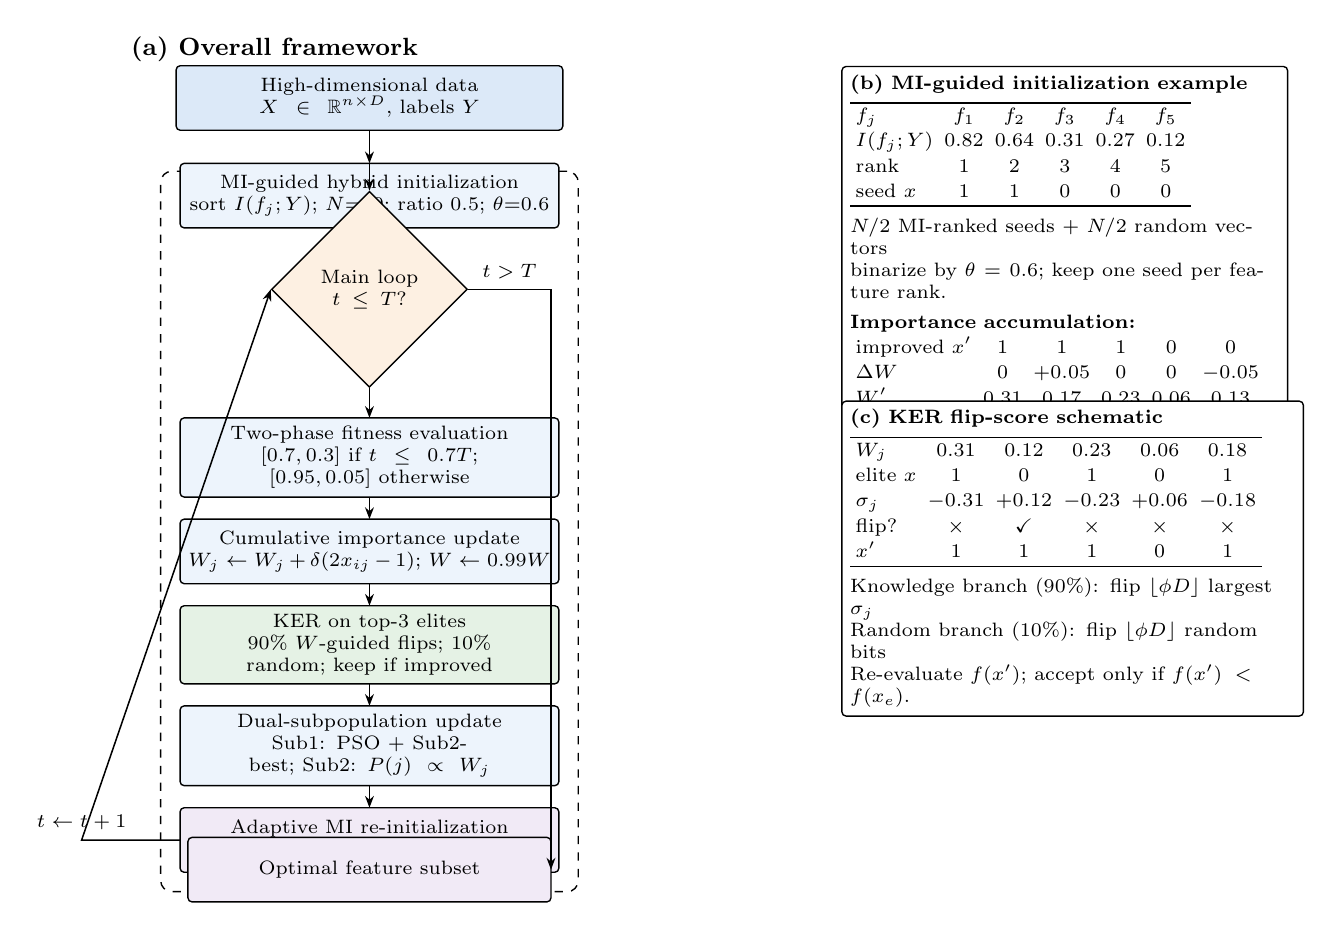
\begin{tikzpicture}[
  font=\scriptsize,
  box/.style={draw, rounded corners=1.5pt, line width=0.5pt, align=center,
              inner sep=3pt, outer sep=0pt},
  flow/.style={box, fill=kblue2, text width=4.6cm, minimum height=0.82cm},
  accent/.style={box, fill=kgreen, text width=4.6cm, minimum height=0.82cm},
  reinit/.style={box, fill=kpurple, text width=4.6cm, minimum height=0.82cm},
  decision/.style={diamond, draw, line width=0.5pt, fill=korange,
                   text width=1.85cm, align=center, inner sep=1pt},
  arrow/.style={-{Stealth[length=1.5mm]}, line width=0.55pt}
]

% ----------------- panel (a): overall framework -----------------
\node[box, fill=kblue, text width=4.7cm, minimum height=0.82cm] (data) at (0,5.45)
  {High-dimensional data\\ $X\in\mathbb{R}^{n\times D}$, labels $Y$};
\node[flow, below=0.42cm of data] (mi)
  {MI-guided hybrid initialization\\ sort $I(f_j;Y)$; $N{=}20$; ratio $0.5$; $\theta{=}0.6$};
\node[decision] (decT) at (0,3.02) {Main loop\\ $t\le T$?};
\node[flow, below=0.38cm of decT] (fitness)
  {Two-phase fitness evaluation\\ $[0.7,0.3]$ if $t\le0.7T$; $[0.95,0.05]$ otherwise};
\node[flow, below=0.28cm of fitness] (wupd)
  {Cumulative importance update\\ $W_j\leftarrow W_j+\delta(2x_{ij}-1)$; $W\leftarrow0.99W$};
\node[accent, below=0.28cm of wupd] (ker)
  {KER on top-3 elites\\ 90\% $W$-guided flips; 10\% random; keep if improved};
\node[flow, below=0.28cm of ker] (update)
  {Dual-subpopulation update\\ Sub1: PSO $+$ Sub2-best; Sub2: $P(j)\propto W_j$};
\node[reinit, below=0.28cm of update] (stall)
  {Adaptive MI re-initialization\\ if stalled $\ge20$ gens, reseed lower half};
\node[box, fill=kpurple, text width=4.4cm, minimum height=0.82cm] (out) at (0,-4.35)
  {Optimal feature subset};

\draw[arrow] (data) -- (mi);
\draw[arrow] (mi) -- (decT);
\draw[arrow] (decT) -- (fitness);
\draw[arrow] (fitness) -- (wupd);
\draw[arrow] (wupd) -- (ker);
\draw[arrow] (ker) -- (update);
\draw[arrow] (update) -- (stall);
\draw[arrow] (decT.east) -| node[above, near start, font=\scriptsize] {$t>T$} (out.east);
\draw[arrow] (stall.west) -- ++(-1.25,0) node[above, font=\scriptsize] {$t\leftarrow t+1$} -- (decT.west);

\node[font=\small\bfseries, anchor=north west] at (-3.15,6.35) {(a) Overall framework};

% dashed loop boundary
\begin{scope}[on background layer]
  \node[draw, dashed, rounded corners=4pt, line width=0.5pt,
        fit=(decT)(fitness)(wupd)(ker)(update)(stall), inner sep=7pt] {};
\end{scope}

% ----------------- panel (b): MI ranking example -----------------
\node[box, fill=white, text width=5.45cm, align=left, anchor=north west] (miEx) at (6.0,5.85)
{%
  \textbf{(b) MI-guided initialization example}\\[2pt]
  \renewcommand{\arraystretch}{1.15}
  \setlength{\tabcolsep}{2pt}
  \begin{tabular}{lccccc}
    \hline
    $f_j$ & $f_1$ & $f_2$ & $f_3$ & $f_4$ & $f_5$\\
    $I(f_j;Y)$ & 0.82 & 0.64 & 0.31 & 0.27 & 0.12\\
    rank & 1 & 2 & 3 & 4 & 5\\
    seed $x$ & 1 & 1 & 0 & 0 & 0\\
    \hline
  \end{tabular}\\[3pt]
  $N/2$ MI-ranked seeds $+$ $N/2$ random vectors\\
  binarize by $\theta=0.6$; keep one seed per feature rank.\\[3pt]
  \textbf{Importance accumulation:}
  \begin{tabular}{lccccc}
    improved $x'$ & 1 & 1 & 1 & 0 & 0\\
    $\Delta W$ & 0 & $+0.05$ & 0 & 0 & $-0.05$\\
    $W'$ & 0.31 & 0.17 & 0.23 & 0.06 & 0.13\\
  \end{tabular}
};

% ----------------- panel (c): KER schematic -----------------
\node[box, fill=white, text width=5.65cm, align=left, anchor=north west] (kerEx) at (6.0,1.6)
{%
  \textbf{(c) KER flip-score schematic}\\[2pt]
  \renewcommand{\arraystretch}{1.15}
  \setlength{\tabcolsep}{2pt}
  \begin{tabular}{lccccc}
    \hline
    $W_j$ & 0.31 & 0.12 & 0.23 & 0.06 & 0.18\\
    elite $x$ & 1 & 0 & 1 & 0 & 1\\
    $\sigma_j$ & $-0.31$ & $+0.12$ & $-0.23$ & $+0.06$ & $-0.18$\\
    flip? & $\times$ & $\checkmark$ & $\times$ & $\times$ & $\times$\\
    $x'$ & 1 & 1 & 1 & 0 & 1\\
    \hline
  \end{tabular}\\[3pt]
  Knowledge branch (90\%): flip $\lfloor\phi D\rfloor$ largest $\sigma_j$\\
  Random branch (10\%): flip $\lfloor\phi D\rfloor$ random bits\\
  Re-evaluate $f(x')$; accept only if $f(x')<f(x_e)$.
};

\end{tikzpicture}
\end{document}
